% !TEX TS-program = pdflatex
% !TEX encoding = UTF-8 Unicode
\documentclass[border=0mm]{standalone}
% packages
\usepackage{tikz}
\usetikzlibrary{patterns}
\usepackage{amsmath,amssymb}
\usepackage{bm}
\usepackage{pgfplots}
\pgfplotsset{compat=1.15}
% start document
\begin{document}
% generated by ROOT (CERN)
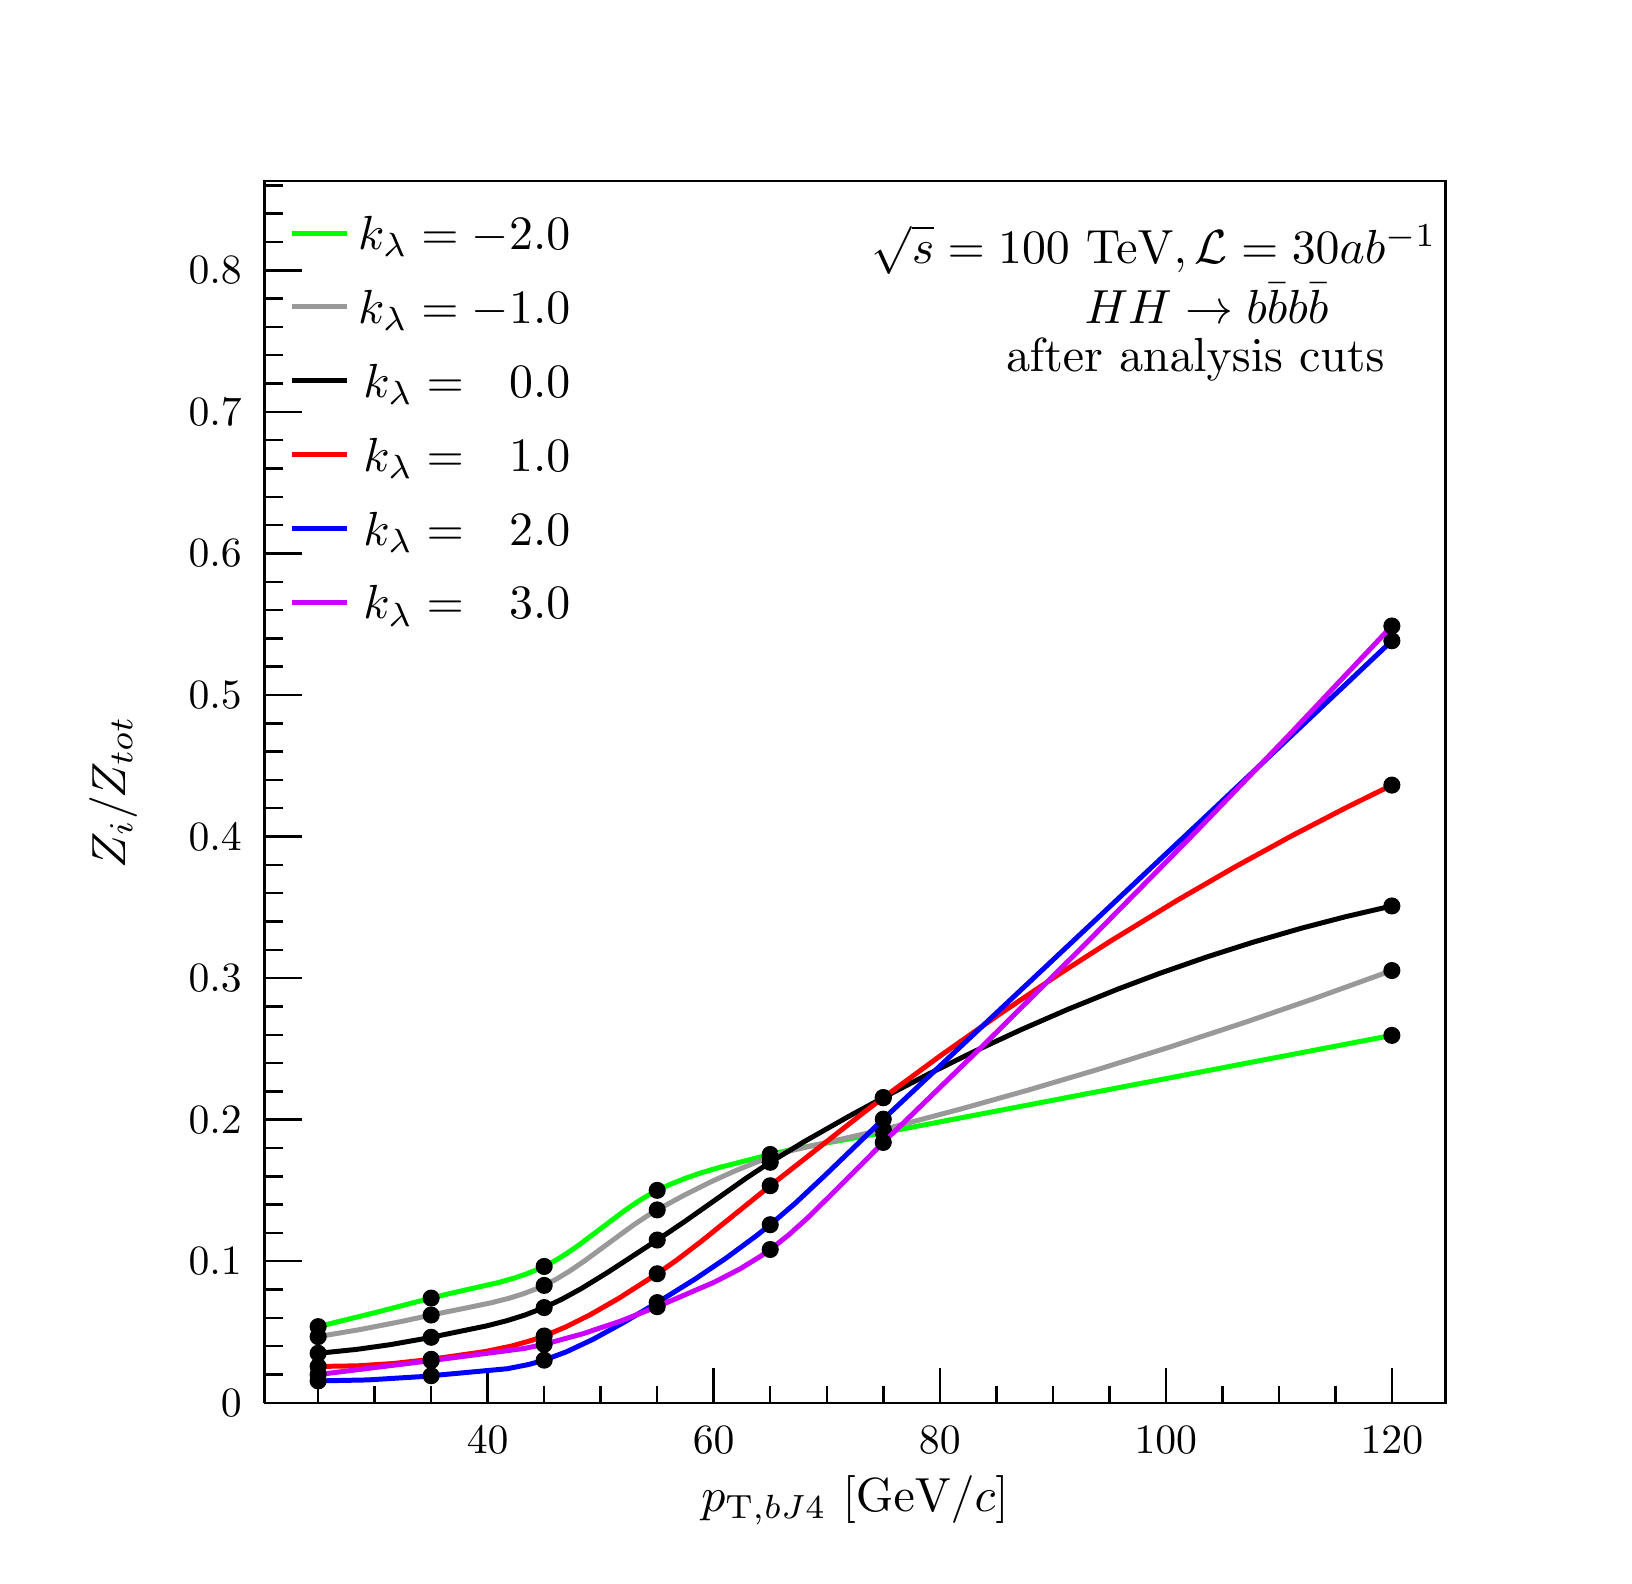
\begin{tikzpicture}
\pgfdeclareplotmark{cross} {
\pgfpathmoveto{\pgfpoint{-0.3\pgfplotmarksize}{\pgfplotmarksize}}
\pgfpathlineto{\pgfpoint{+0.3\pgfplotmarksize}{\pgfplotmarksize}}
\pgfpathlineto{\pgfpoint{+0.3\pgfplotmarksize}{0.3\pgfplotmarksize}}
\pgfpathlineto{\pgfpoint{+1\pgfplotmarksize}{0.3\pgfplotmarksize}}
\pgfpathlineto{\pgfpoint{+1\pgfplotmarksize}{-0.3\pgfplotmarksize}}
\pgfpathlineto{\pgfpoint{+0.3\pgfplotmarksize}{-0.3\pgfplotmarksize}}
\pgfpathlineto{\pgfpoint{+0.3\pgfplotmarksize}{-1.\pgfplotmarksize}}
\pgfpathlineto{\pgfpoint{-0.3\pgfplotmarksize}{-1.\pgfplotmarksize}}
\pgfpathlineto{\pgfpoint{-0.3\pgfplotmarksize}{-0.3\pgfplotmarksize}}
\pgfpathlineto{\pgfpoint{-1.\pgfplotmarksize}{-0.3\pgfplotmarksize}}
\pgfpathlineto{\pgfpoint{-1.\pgfplotmarksize}{0.3\pgfplotmarksize}}
\pgfpathlineto{\pgfpoint{-0.3\pgfplotmarksize}{0.3\pgfplotmarksize}}
\pgfpathclose
\pgfusepathqstroke
}
\pgfdeclareplotmark{cross*} {
\pgfpathmoveto{\pgfpoint{-0.3\pgfplotmarksize}{\pgfplotmarksize}}
\pgfpathlineto{\pgfpoint{+0.3\pgfplotmarksize}{\pgfplotmarksize}}
\pgfpathlineto{\pgfpoint{+0.3\pgfplotmarksize}{0.3\pgfplotmarksize}}
\pgfpathlineto{\pgfpoint{+1\pgfplotmarksize}{0.3\pgfplotmarksize}}
\pgfpathlineto{\pgfpoint{+1\pgfplotmarksize}{-0.3\pgfplotmarksize}}
\pgfpathlineto{\pgfpoint{+0.3\pgfplotmarksize}{-0.3\pgfplotmarksize}}
\pgfpathlineto{\pgfpoint{+0.3\pgfplotmarksize}{-1.\pgfplotmarksize}}
\pgfpathlineto{\pgfpoint{-0.3\pgfplotmarksize}{-1.\pgfplotmarksize}}
\pgfpathlineto{\pgfpoint{-0.3\pgfplotmarksize}{-0.3\pgfplotmarksize}}
\pgfpathlineto{\pgfpoint{-1.\pgfplotmarksize}{-0.3\pgfplotmarksize}}
\pgfpathlineto{\pgfpoint{-1.\pgfplotmarksize}{0.3\pgfplotmarksize}}
\pgfpathlineto{\pgfpoint{-0.3\pgfplotmarksize}{0.3\pgfplotmarksize}}
\pgfpathclose
\pgfusepathqfillstroke
}
\pgfdeclareplotmark{newstar} {
\pgfpathmoveto{\pgfqpoint{0pt}{\pgfplotmarksize}}
\pgfpathlineto{\pgfqpointpolar{44}{0.5\pgfplotmarksize}}
\pgfpathlineto{\pgfqpointpolar{18}{\pgfplotmarksize}}
\pgfpathlineto{\pgfqpointpolar{-20}{0.5\pgfplotmarksize}}
\pgfpathlineto{\pgfqpointpolar{-54}{\pgfplotmarksize}}
\pgfpathlineto{\pgfqpointpolar{-90}{0.5\pgfplotmarksize}}
\pgfpathlineto{\pgfqpointpolar{234}{\pgfplotmarksize}}
\pgfpathlineto{\pgfqpointpolar{198}{0.5\pgfplotmarksize}}
\pgfpathlineto{\pgfqpointpolar{162}{\pgfplotmarksize}}
\pgfpathlineto{\pgfqpointpolar{134}{0.5\pgfplotmarksize}}
\pgfpathclose
\pgfusepathqstroke
}
\pgfdeclareplotmark{newstar*} {
\pgfpathmoveto{\pgfqpoint{0pt}{\pgfplotmarksize}}
\pgfpathlineto{\pgfqpointpolar{44}{0.5\pgfplotmarksize}}
\pgfpathlineto{\pgfqpointpolar{18}{\pgfplotmarksize}}
\pgfpathlineto{\pgfqpointpolar{-20}{0.5\pgfplotmarksize}}
\pgfpathlineto{\pgfqpointpolar{-54}{\pgfplotmarksize}}
\pgfpathlineto{\pgfqpointpolar{-90}{0.5\pgfplotmarksize}}
\pgfpathlineto{\pgfqpointpolar{234}{\pgfplotmarksize}}
\pgfpathlineto{\pgfqpointpolar{198}{0.5\pgfplotmarksize}}
\pgfpathlineto{\pgfqpointpolar{162}{\pgfplotmarksize}}
\pgfpathlineto{\pgfqpointpolar{134}{0.5\pgfplotmarksize}}
\pgfpathclose
\pgfusepathqfillstroke
}
\definecolor{c}{rgb}{1,1,1};
\draw [color=c, fill=c] (0,0) rectangle (20,19.397);
\draw [color=c, fill=c] (3,1.9397) rectangle (18,17.4573);
\definecolor{c}{rgb}{0,0,0};
\draw [c,line width=0.9] (3,1.9397) -- (3,17.4573) -- (18,17.4573) -- (18,1.9397) -- (3,1.9397);
\definecolor{c}{rgb}{1,1,1};
\draw [color=c, fill=c] (3,1.9397) rectangle (18,17.4573);
\definecolor{c}{rgb}{0,0,0};
\draw [c,line width=0.9] (3,1.9397) -- (3,17.4573) -- (18,17.4573) -- (18,1.9397) -- (3,1.9397);
\draw [c,line width=0.9] (3,1.9397) -- (18,1.9397);
\draw [c,line width=0.9] (5.83493,2.37613) -- (5.83493,1.9397);
\draw [c,line width=0.9] (6.55263,2.15791) -- (6.55263,1.9397);
\draw [c,line width=0.9] (7.27034,2.15791) -- (7.27034,1.9397);
\draw [c,line width=0.9] (7.98804,2.15791) -- (7.98804,1.9397);
\draw [c,line width=0.9] (8.70574,2.37613) -- (8.70574,1.9397);
\draw [c,line width=0.9] (9.42344,2.15791) -- (9.42344,1.9397);
\draw [c,line width=0.9] (10.1411,2.15791) -- (10.1411,1.9397);
\draw [c,line width=0.9] (10.8589,2.15791) -- (10.8589,1.9397);
\draw [c,line width=0.9] (11.5766,2.37613) -- (11.5766,1.9397);
\draw [c,line width=0.9] (12.2943,2.15791) -- (12.2943,1.9397);
\draw [c,line width=0.9] (13.012,2.15791) -- (13.012,1.9397);
\draw [c,line width=0.9] (13.7297,2.15791) -- (13.7297,1.9397);
\draw [c,line width=0.9] (14.4474,2.37613) -- (14.4474,1.9397);
\draw [c,line width=0.9] (15.1651,2.15791) -- (15.1651,1.9397);
\draw [c,line width=0.9] (15.8828,2.15791) -- (15.8828,1.9397);
\draw [c,line width=0.9] (16.6005,2.15791) -- (16.6005,1.9397);
\draw [c,line width=0.9] (17.3182,2.37613) -- (17.3182,1.9397);
\draw [c,line width=0.9] (5.83493,2.37613) -- (5.83493,1.9397);
\draw [c,line width=0.9] (5.11723,2.15791) -- (5.11723,1.9397);
\draw [c,line width=0.9] (4.39952,2.15791) -- (4.39952,1.9397);
\draw [c,line width=0.9] (3.68182,2.15791) -- (3.68182,1.9397);
\draw [c,line width=0.9] (17.3182,2.37613) -- (17.3182,1.9397);
\draw [anchor=base] (5.83493,1.2996) node[scale=1.50669, color=c, rotate=0]{40};
\draw [anchor=base] (8.70574,1.2996) node[scale=1.50669, color=c, rotate=0]{60};
\draw [anchor=base] (11.5766,1.2996) node[scale=1.50669, color=c, rotate=0]{80};
\draw [anchor=base] (14.4474,1.2996) node[scale=1.50669, color=c, rotate=0]{100};
\draw [anchor=base] (17.3182,1.2996) node[scale=1.50669, color=c, rotate=0]{120};
\draw (10.5,0.698292) node[scale=1.7299, color=c, rotate=0]{$p_{\text{T},bJ4} ~[\text{GeV}/c]$};
\draw [c,line width=0.9] (3,1.9397) -- (3,17.4573);
\draw [c,line width=0.9] (3.48,1.9397) -- (3,1.9397);
\draw [c,line width=0.9] (3.24,2.29926) -- (3,2.29926);
\draw [c,line width=0.9] (3.24,2.65883) -- (3,2.65883);
\draw [c,line width=0.9] (3.24,3.01839) -- (3,3.01839);
\draw [c,line width=0.9] (3.24,3.37795) -- (3,3.37795);
\draw [c,line width=0.9] (3.48,3.73752) -- (3,3.73752);
\draw [c,line width=0.9] (3.24,4.09708) -- (3,4.09708);
\draw [c,line width=0.9] (3.24,4.45665) -- (3,4.45665);
\draw [c,line width=0.9] (3.24,4.81621) -- (3,4.81621);
\draw [c,line width=0.9] (3.24,5.17577) -- (3,5.17577);
\draw [c,line width=0.9] (3.48,5.53534) -- (3,5.53534);
\draw [c,line width=0.9] (3.24,5.8949) -- (3,5.8949);
\draw [c,line width=0.9] (3.24,6.25447) -- (3,6.25447);
\draw [c,line width=0.9] (3.24,6.61403) -- (3,6.61403);
\draw [c,line width=0.9] (3.24,6.97359) -- (3,6.97359);
\draw [c,line width=0.9] (3.48,7.33316) -- (3,7.33316);
\draw [c,line width=0.9] (3.24,7.69272) -- (3,7.69272);
\draw [c,line width=0.9] (3.24,8.05228) -- (3,8.05228);
\draw [c,line width=0.9] (3.24,8.41185) -- (3,8.41185);
\draw [c,line width=0.9] (3.24,8.77141) -- (3,8.77141);
\draw [c,line width=0.9] (3.48,9.13098) -- (3,9.13098);
\draw [c,line width=0.9] (3.24,9.49054) -- (3,9.49054);
\draw [c,line width=0.9] (3.24,9.8501) -- (3,9.8501);
\draw [c,line width=0.9] (3.24,10.2097) -- (3,10.2097);
\draw [c,line width=0.9] (3.24,10.5692) -- (3,10.5692);
\draw [c,line width=0.9] (3.48,10.9288) -- (3,10.9288);
\draw [c,line width=0.9] (3.24,11.2884) -- (3,11.2884);
\draw [c,line width=0.9] (3.24,11.6479) -- (3,11.6479);
\draw [c,line width=0.9] (3.24,12.0075) -- (3,12.0075);
\draw [c,line width=0.9] (3.24,12.3671) -- (3,12.3671);
\draw [c,line width=0.9] (3.48,12.7266) -- (3,12.7266);
\draw [c,line width=0.9] (3.24,13.0862) -- (3,13.0862);
\draw [c,line width=0.9] (3.24,13.4457) -- (3,13.4457);
\draw [c,line width=0.9] (3.24,13.8053) -- (3,13.8053);
\draw [c,line width=0.9] (3.24,14.1649) -- (3,14.1649);
\draw [c,line width=0.9] (3.48,14.5244) -- (3,14.5244);
\draw [c,line width=0.9] (3.24,14.884) -- (3,14.884);
\draw [c,line width=0.9] (3.24,15.2436) -- (3,15.2436);
\draw [c,line width=0.9] (3.24,15.6031) -- (3,15.6031);
\draw [c,line width=0.9] (3.24,15.9627) -- (3,15.9627);
\draw [c,line width=0.9] (3.48,16.3223) -- (3,16.3223);
\draw [c,line width=0.9] (3.48,16.3223) -- (3,16.3223);
\draw [c,line width=0.9] (3.24,16.6818) -- (3,16.6818);
\draw [c,line width=0.9] (3.24,17.0414) -- (3,17.0414);
\draw [c,line width=0.9] (3.24,17.4009) -- (3,17.4009);
\draw [anchor= east] (2.9,1.9397) node[scale=1.50669, color=c, rotate=0]{0};
\draw [anchor= east] (2.9,3.73752) node[scale=1.50669, color=c, rotate=0]{0.1};
\draw [anchor= east] (2.9,5.53534) node[scale=1.50669, color=c, rotate=0]{0.2};
\draw [anchor= east] (2.9,7.33316) node[scale=1.50669, color=c, rotate=0]{0.3};
\draw [anchor= east] (2.9,9.13098) node[scale=1.50669, color=c, rotate=0]{0.4};
\draw [anchor= east] (2.9,10.9288) node[scale=1.50669, color=c, rotate=0]{0.5};
\draw [anchor= east] (2.9,12.7266) node[scale=1.50669, color=c, rotate=0]{0.6};
\draw [anchor= east] (2.9,14.5244) node[scale=1.50669, color=c, rotate=0]{0.7};
\draw [anchor= east] (2.9,16.3223) node[scale=1.50669, color=c, rotate=0]{0.8};
\draw (1.08,9.69849) node[scale=1.7299, color=c, rotate=90]{$Z_{i}/Z_{tot}$};
\definecolor{c}{rgb}{0,1,0};
\draw [c,line width=1.8] (3.68182,2.907) -- (4.42387,3.08982) -- (5.11723,3.26996) -- (5.34211,3.32493) -- (5.97941,3.46894) -- (6.17156,3.52375) -- (6.327,3.57665) -- (6.48135,3.6389) -- (6.55263,3.67146) -- (6.67753,3.73668) -- (6.8197,3.82339) --
 (7.0021,3.94928) -- (7.30934,4.18124) -- (7.58872,4.39056) -- (7.73161,4.48891) -- (7.8586,4.56793) -- (7.98804,4.63798) -- (8.1626,4.71835) -- (8.36314,4.7977) -- (8.54995,4.8614) -- (8.76429,4.92525) -- (9.42344,5.09354) -- (9.73453,5.16538) --
 (10.8589,5.37015) -- (17.3182,6.60599);
\definecolor{c}{rgb}{0,0,0};
\foreach \P in {(3.68182,2.907), (5.11723,3.26996), (6.55263,3.67146), (7.98804,4.63798), (9.42344,5.09354), (10.8589,5.37015), (17.3182,6.60599)}{\draw[mark options={color=c,fill=c},mark size=2.882883pt,mark=*] plot coordinates {\P};}
\definecolor{c}{rgb}{0.6,0.6,0.6};
\draw [c,line width=1.8] (3.68182,2.78032) -- (4.20973,2.86938) -- (4.72868,2.97036) -- (5.11723,3.05467) -- (5.57121,3.14631) -- (5.88214,3.21078) -- (6.10621,3.26767) -- (6.2853,3.32359) -- (6.46098,3.3904) -- (6.55263,3.43084) -- (6.70408,3.50872)
 -- (6.87658,3.61326) -- (7.06466,3.74139) -- (7.37366,3.96878) -- (7.67723,4.1905) -- (7.85368,4.3087) -- (7.98804,4.38968) -- (8.31681,4.56942) -- (8.67597,4.74915) -- (8.96325,4.87937) -- (9.25102,4.99683) -- (9.42344,5.06064) -- (9.6513,5.13377)
 -- (10.8589,5.41032) -- (11.8486,5.67241) -- (12.6902,5.90871) -- (13.5934,6.17612) -- (14.4915,6.45615) -- (15.4521,6.77129) -- (16.3024,7.06368) -- (17.3182,7.42963);
\definecolor{c}{rgb}{0,0,0};
\foreach \P in {(3.68182,2.78032), (5.11723,3.05467), (6.55263,3.43084), (7.98804,4.38968), (9.42344,5.06064), (10.8589,5.41032), (17.3182,7.42963)}{\draw[mark options={color=c,fill=c},mark size=2.882883pt,mark=*] plot coordinates {\P};}
\draw [c,line width=1.8] (3.68182,2.56843) -- (4.16799,2.6179) -- (4.59586,2.67793) -- (5.04633,2.7578) -- (5.11723,2.77193) -- (5.82718,2.91792) -- (6.08593,2.98485) -- (6.31129,3.05583) -- (6.55263,3.14921) -- (6.77882,3.2561) -- (7.02833,3.39307)
 -- (7.36287,3.59869) -- (7.98804,4.00715) -- (8.32685,4.23481) -- (9.12837,4.8001) -- (9.42344,4.99442) -- (9.85105,5.25434) -- (10.428,5.58163) -- (10.8589,5.81531) -- (11.4343,6.11577) -- (12.0183,6.40394) -- (12.6083,6.67794) -- (13.1988,6.935)
 -- (13.83,7.19069) -- (14.367,7.39276) -- (14.9623,7.60017) -- (15.5537,7.78893) -- (16.1671,7.96645) -- (16.7298,8.11306) -- (17.3182,8.24964);
\foreach \P in {(3.68182,2.56843), (5.11723,2.77193), (6.55263,3.14921), (7.98804,4.00715), (9.42344,4.99442), (10.8589,5.81531), (17.3182,8.24964)}{\draw[mark options={color=c,fill=c},mark size=2.882883pt,mark=*] plot coordinates {\P};}
\definecolor{c}{rgb}{1,0,0};
\draw [c,line width=1.8] (3.68182,2.40116) -- (4.1776,2.4094) -- (4.62808,2.43809) -- (5.11723,2.49212) -- (5.81256,2.59244) -- (6.14455,2.66209) -- (6.40614,2.73665) -- (6.55263,2.78814) -- (6.82758,2.90372) -- (7.13196,3.05577) -- (7.49721,3.2651)
 -- (7.98804,3.57867) -- (8.23919,3.75471) -- (8.54812,3.99098) -- (9.42344,4.69645) -- (10.6133,5.62867) -- (10.8589,5.81499) -- (11.5912,6.35252) -- (12.3232,6.86736) -- (13.0888,7.38199) -- (13.7404,7.80074) -- (14.5756,8.31153) --
 (15.3084,8.73576) -- (16.0388,9.13637) -- (16.7483,9.50425) -- (17.3182,9.78456);
\definecolor{c}{rgb}{0,0,0};
\foreach \P in {(3.68182,2.40116), (5.11723,2.49212), (6.55263,2.78814), (7.98804,3.57867), (9.42344,4.69645), (10.8589,5.81499), (17.3182,9.78456)}{\draw[mark options={color=c,fill=c},mark size=2.882883pt,mark=*] plot coordinates {\P};}
\definecolor{c}{rgb}{0,0,1};
\draw [c,line width=1.8] (3.68182,2.21774) -- (4.31307,2.23048) -- (4.97928,2.27161) -- (5.11723,2.28368) -- (6.08277,2.37264) -- (6.35956,2.42713) -- (6.55263,2.48161) -- (6.83856,2.589) -- (7.17367,2.74688) -- (7.57101,2.96513) -- (7.98804,3.21228)
 -- (8.47132,3.51297) -- (8.8623,3.77727) -- (9.24951,4.06349) -- (9.42344,4.20144) -- (9.74227,4.47546) -- (10.1281,4.83686) -- (10.8589,5.54187) -- (14.8723,9.30852) -- (17.3182,11.6175);
\definecolor{c}{rgb}{0,0,0};
\foreach \P in {(3.68182,2.21774), (5.11723,2.28368), (6.55263,2.48161), (7.98804,3.21228), (9.42344,4.20144), (10.8589,5.54187), (17.3182,11.6175)}{\draw[mark options={color=c,fill=c},mark size=2.882883pt,mark=*] plot coordinates {\P};}
\definecolor{c}{rgb}{0.8,0,1};
\draw [c,line width=1.8] (3.68182,2.2984) -- (5.11723,2.47578) -- (6.30474,2.63078) -- (6.55263,2.6829) -- (7.05028,2.81868) -- (7.51646,2.97533) -- (7.98804,3.16045) -- (8.71262,3.47187) -- (9.04045,3.64122) -- (9.30196,3.80214) -- (9.42344,3.88685)
 -- (9.65651,4.07105) -- (9.89365,4.28388) -- (10.2677,4.65229) -- (10.8589,5.24634) -- (12.1598,6.50924) -- (13.452,7.79267) -- (14.7941,9.15628) -- (16.0225,10.4318) -- (17.3182,11.8054);
\definecolor{c}{rgb}{0,0,0};
\foreach \P in {(3.68182,2.2984), (5.11723,2.47578), (6.55263,2.6829), (7.98804,3.16045), (9.42344,3.88685), (10.8589,5.24634), (17.3182,11.8054)}{\draw[mark options={color=c,fill=c},mark size=2.882883pt,mark=*] plot coordinates {\P};}
\draw [anchor= west] (10.5,16.5844) node[scale=1.7299, color=c, rotate=0]{$\sqrt{s} = 100 ~\text{TeV}, \mathcal{L} = 30 ab^{-1}$};
\draw [anchor= west] (13.2,15.9055) node[scale=1.7299, color=c, rotate=0]{$HH \rightarrow b\bar{b}b\bar{b}$};
\draw [anchor=base west] (12.2,15.0424) node[scale=1.7299, color=c, rotate=0]{after analysis cuts};
\draw [anchor=base east] (7.1,16.5836) node[scale=1.7299, color=c, rotate=0]{$k_{\lambda} = -2.0$};
\definecolor{c}{rgb}{0,1,0};
\draw [c,line width=1.8] (3.35,16.7946) -- (4.05,16.7946);
\definecolor{c}{rgb}{0,0,0};
\draw [anchor=base east] (7.1,15.6461) node[scale=1.7299, color=c, rotate=0]{$k_{\lambda} = -1.0$};
\definecolor{c}{rgb}{0.6,0.6,0.6};
\draw [c,line width=1.8] (3.35,15.857) -- (4.05,15.857);
\definecolor{c}{rgb}{0,0,0};
\draw [anchor=base east] (7.1,14.7086) node[scale=1.7299, color=c, rotate=0]{$k_{\lambda} =~~0.0$};
\draw [c,line width=1.8] (3.35,14.9195) -- (4.05,14.9195);
\draw [anchor=base east] (7.1,13.7711) node[scale=1.7299, color=c, rotate=0]{$k_{\lambda} =~~1.0$};
\definecolor{c}{rgb}{1,0,0};
\draw [c,line width=1.8] (3.35,13.982) -- (4.05,13.982);
\definecolor{c}{rgb}{0,0,0};
\draw [anchor=base east] (7.1,12.8335) node[scale=1.7299, color=c, rotate=0]{$k_{\lambda} =~~2.0$};
\definecolor{c}{rgb}{0,0,1};
\draw [c,line width=1.8] (3.35,13.0445) -- (4.05,13.0445);
\definecolor{c}{rgb}{0,0,0};
\draw [anchor=base east] (7.1,11.896) node[scale=1.7299, color=c, rotate=0]{$k_{\lambda} =~~3.0$};
\definecolor{c}{rgb}{0.8,0,1};
\draw [c,line width=1.8] (3.35,12.107) -- (4.05,12.107);
\end{tikzpicture}
% end document
\end{document}
